\section{Introduction}

This work is dedicated to developing an architecture for solving DensePose \cite{densepose} estimation task with a particular requirement: the model should be light-weight and run in real-time on a mobile device.

The task of understanding humans in an image may involve different formulations of the problem: 2d landmarks localization, human part segmentation, 3d reconstruction, dense image-to-surface correspondences (DensePose). In this work, we target the multi-person formulation of DensePose task: given a single RGB image solve the regression task: for each pixel, find its surface points (UV coordinates) on a deformable surface model (the Skinned Multi-Person Linear (SMPL) model \cite{smpl}).

Finding surface correspondence is a step forward to a general 3d human representation. Possible applications lie in such fields, like augmented reality, virtual fitting rooms. Densepose output may serve as input to another model. For instance, it was used as an input in video-to-video translation tasks \cite{vid2vid}.

Besides the original pioneering work \cite{densepose}, which introduces a carefully annotated COCO-DensePose dataset with sparse image-to-surface ground-truth correspondences and DensePose R-CNN baseline model, other works target different formulations. Parsing R-CNN \cite{parsing}, the winner solution of the COCO 2018 Challenge DensePose Estimation task, achieves state-of-the-art performance by scrutinizing different blocks in the original DensePose R-CNN architecture. Slim DensePose \cite{denseposeslim} explores the weakly-supervised and self-supervised learning problem setting, by leveraging motion cues from videos. \cite{uncertainty} improves the performance of the model by incorporating the uncertainty estimation into the model. \cite{monkeys} shows the ability to transfer the dense pose recognition from humans to proximal animal classes such as chimpanzees without a time-consuming collection of a new dataset with new classes.

However, none of the works target the task of making the network fast and light-weight, and current solutions such as baseline DensePose R-CNN and state-of-the-art Parsing R-CNN introduce heavily parametrized models.

Make the network perform near to a real-time mode is a particularly important step if we want to apply these models in the mobile or embedded devices. In this work, we explore the subtle trade-off between the performance of the 
model and its latency.

\noindent \textbf{Model architecture optimisation.}
In recent years the neural architecture search (NAS) techniques gained popularity \cite{automl}. The main aim of NAS is to find the optimal architecture under specific hardware requirements. Usually, these techniques are applied in simple setups, e.g., classification networks, or in the case of two-stage object detection models, NAS is usually applied to individual parts of the model \cite{nasfpn}. In this paper, instead of creating one more design for a particular part of the model, we try to test different existing approaches and see what works best for the DensePose estimation task. Particularly, we evaluate several backbones that were a result of NAS optimization and try to test them out with other components.

\begin{figure}[!hbtp]
\centering
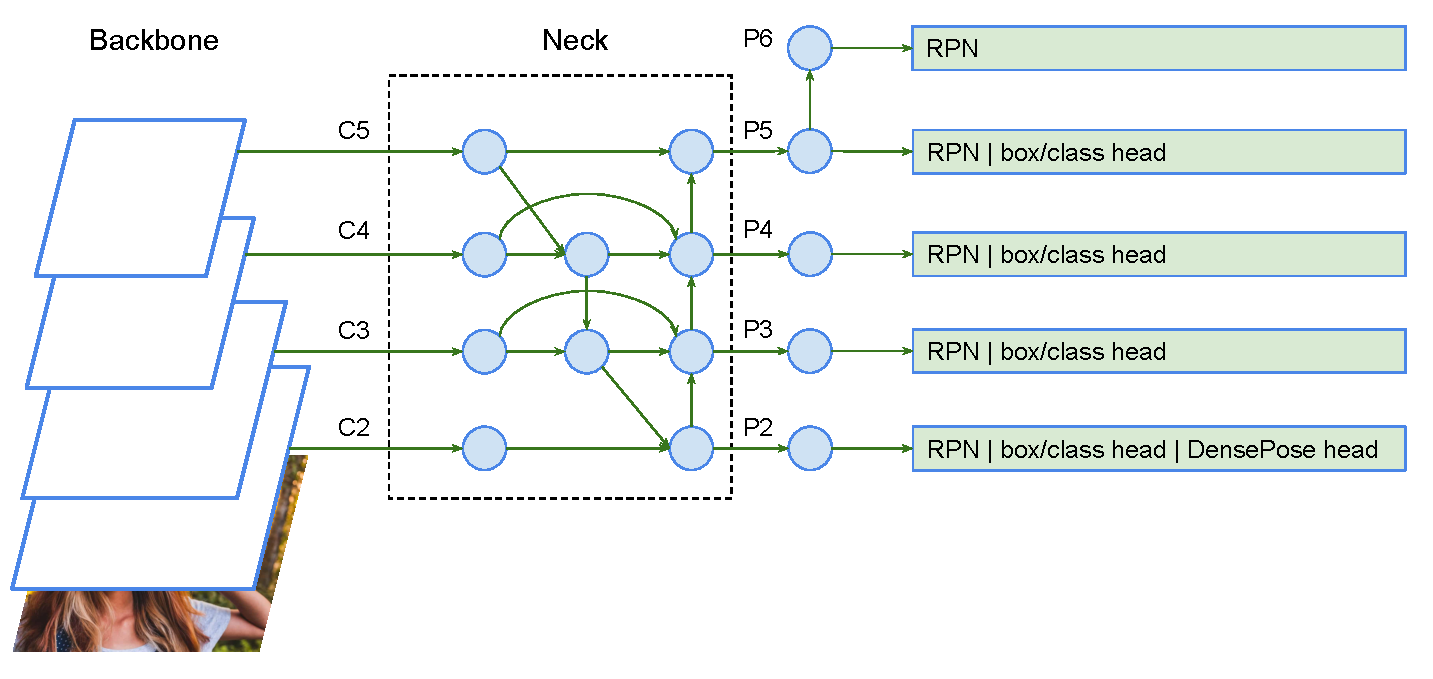
\includegraphics[width=0.4\textwidth]{Figures/densepose/scheme.pdf}
\caption{The high level structure of the Mobile Parsing R-CNN model. $C_i$, $P_i$ represent feature levels with a resolution of $1/2^i$ of the input image. $P_6$ is obtained via stride-2 pooling on $P_5$.}
\label{fig:scheme}
\end{figure}

The contributions are the following:
\begin{itemize}
    \item we created a pipeline to test neural network architectures viability for mobile deployment,
    \item we developed an architecture based on existing techniques, achieving a finally good balance between real-time speed and average precision of our model,
    \item we performed an ablation study on many different efficient backbones, particularly applied for DensePose task.
\end{itemize}